%\selectlanguage{czech}
\chapter{Webová aplikace - Pulley systems simulation}
\label{Webova_aplikace}
%% -------------------------------------------------- %%
\def\figurename{Obr.} % Figure name
\def\tablename{Tab.} % Table name
\def\figureautorefname{obr.} % Autoreference 
\def\tableautorefname{tab.} % Autoreference
\def\chapterautorefname{kapitola} % Autoreference
%% -------------------------------------------------- %%

\section{Představení aplikace}

Vytvořila jsem webovou aplikaci, pro výpočet potřebné síly k vytažení zachraňovaného lezce (viz~\autoref{Obr:1_application}). První volbou v aplikaci je požadovaný systém kladkostroje, který se v zápětí vykreslí (viz~\autoref{Obr:6_application}). Lze zvolit kladkostroje s mechanickou účinností 3:1, 5:1 a nebo 7:1 (viz~\autoref{Obr:2_application}). Druhou volbou v aplikaci je nastavení konkrétní účinnosti jednotlivých kladek v systému (viz~\autoref{Obr:3_application}). Pokud není nastavena žádná hodnota, uvažuje se se 100\% účinností, jedná se o dokonalý stav, který v realném prostředí není možný. Pomocí posuvníku či příslušných tlačítek lze nastavit hmotnost lezce (viz~\autoref{Obr:4_application}). V neposlední řadě lze nastavit vzdálenost, kterou chceme za pomocí kladkostroje překonat (viz~\autoref{Obr:5_application}). 

%% -------------------------------------------------- %%
%% -------------------- Picture --------------------- %%
%% -------------------------------------------------- %%
\begin{figure}[!hbt]
    \centering
    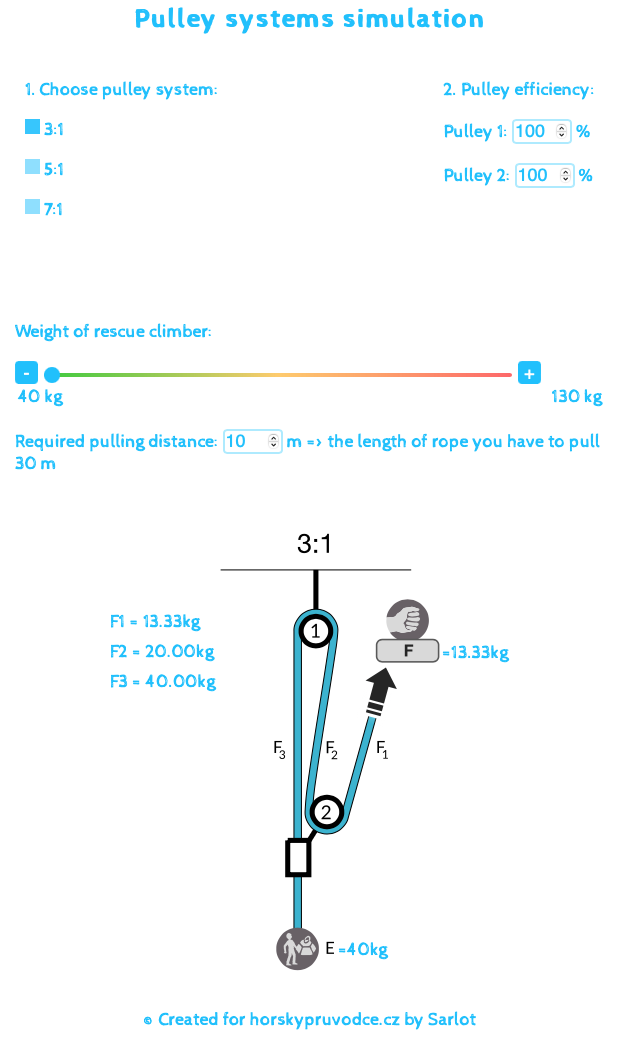
\includegraphics[width=10.0cm]{Figures/WebApplication/1_Web_application.png}
    \caption[1_Aplikace]{Kompletní zobrazení aplikace}
    \label{Obr:1_application}
\end{figure} 
%% -------------------------------------------------- %%

%% -------------------------------------------------- %%
%% -------------------- Picture --------------------- %%
%% -------------------------------------------------- %%
\begin{figure}[!hbt]
    \centering
    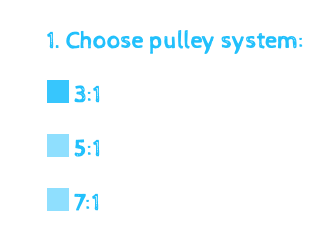
\includegraphics[width=4.0cm]{Figures/WebApplication/2_Web_application.png}
    \caption[2_Aplikace]{První volba v aplikaci - výběr kladkostroje}
    \label{Obr:2_application}
\end{figure} 
%% -------------------------------------------------- %%

%% -------------------------------------------------- %%
%% -------------------- Picture --------------------- %%
%% -------------------------------------------------- %%
\begin{figure}[!hbt]
    \centering
    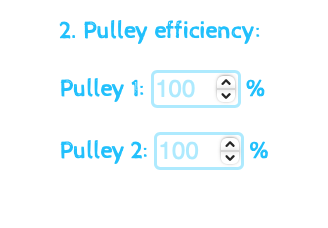
\includegraphics[width=4.0cm]{Figures/WebApplication/3_Web_application.png}
    \caption[3_Aplikace]{Možnost nastavit konkrétní hodnotu účinnosti dané kladky}
    \label{Obr:3_application}
\end{figure} 
%% -------------------------------------------------- %%

%% -------------------------------------------------- %%
%% -------------------- Picture --------------------- %%
%% -------------------------------------------------- %%
\begin{figure}[!hbt]
    \centering
    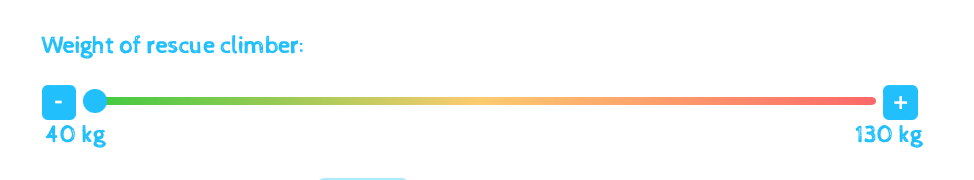
\includegraphics[width=10.0cm]{Figures/WebApplication/4_Web_application.png}
    \caption[4_Aplikace]{Nastavení hmotnosti vytahovaného lezce}
    \label{Obr:4_application}
\end{figure} 
%% -------------------------------------------------- %%

%% -------------------------------------------------- %%
%% -------------------- Picture --------------------- %%
%% -------------------------------------------------- %%
\begin{figure}[!hbt]
    \centering
    
\includegraphics[width=10.0cm]{Figures/WebApplication/5_Web_application.png}
    \caption[5_Aplikace]{Zadání požadované vzdálenosti vytahovaného lezce}
    \label{Obr:5_application}
\end{figure} 
%% -------------------------------------------------- %%

%% -------------------------------------------------- %%
%% -------------------- Picture --------------------- %%
%% -------------------------------------------------- %%
\begin{figure}[!hbt]
    \centering
    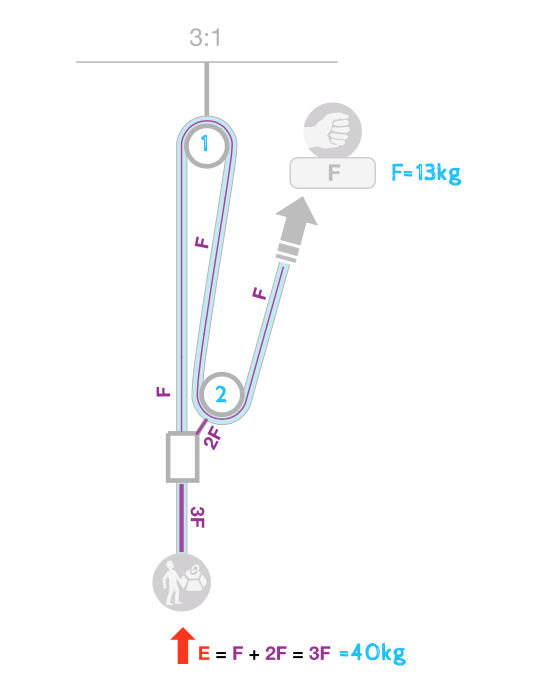
\includegraphics[width=8.0cm]{Figures/WebApplication/6_Web_application.png}
    \caption[6_Aplikace]{Schéma kladkostroje}
    \label{Obr:6_application}
\end{figure} 
%% -------------------------------------------------- %%